\chapter{ระเบียบวิธีดำเนินโครงงาน}
\label{Ch:Methodology}

โครงงานนี้มีวัตถุประสงค์เพื่อพัฒนาไลบรารีสำหรับตรวจจับ {\italicfont Green Code Smell} ในภาษา Python ควบคู่กับการพัฒนาส่วนขยาย {\italicfont Visual Studio Code (VS Code Extension)} เพื่อใช้ในการวิเคราะห์ แสดงผล และประเมินผลกระทบด้านพลังงานและคาร์บอนของโค้ดอย่างเป็นระบบ โดยในฉบับปรับปรุงนี้ ได้มีการเพิ่มขีดความสามารถด้านมาตรวัดเชิงฟังก์ชัน ({\italicfont Functional Metrics}) และการวิเคราะห์ผลกระทบเชิงประจักษ์ เพื่อให้ระบบสามารถสะท้อนผลของการปรับปรุงโค้ดได้ชัดเจนยิ่งขึ้น

% -----------------------------------------------------

\section{การวางแผนและองค์ประกอบของระบบ}

การพัฒนาระบบประกอบด้วยองค์ประกอบหลัก 5 ส่วน ได้แก่ AST Parser, ชุดกฎสำหรับตรวจจับ Green Code Smell, Metric and Analysis Module, VS Code Extension Module และ Reporting Module ดังนี้

\begin{itemize}
    \item AST Parser
    \item ชุดกฎสำหรับตรวจจับ Green Code Smell
    \item Metric and Analysis Module
    \item VS Code Extension Module
    \item Reporting Module
\end{itemize}

\subsection{สถาปัตยกรรมภาพรวมของระบบ}
จากองค์ประกอบทั้ง 5 ส่วนดังกล่าว ระบบถูกออกแบบให้ทำงานเป็นลำดับตั้งแต่การแปลงซอร์สโค้ดให้เป็น AST การตรวจจับ Green Code Smell การคำนวณมาตรวัดเชิงฟังก์ชันและผลกระทบด้านคาร์บอน ไปจนถึงการแสดงผลผ่านส่วนขยาย VS Code และการส่งออกผลลัพธ์ในรูปแบบ log/JSON ดังแสดงในรูป \ref{fig:ch4_overall_architecture}

\begin{figure}[H]
\centering
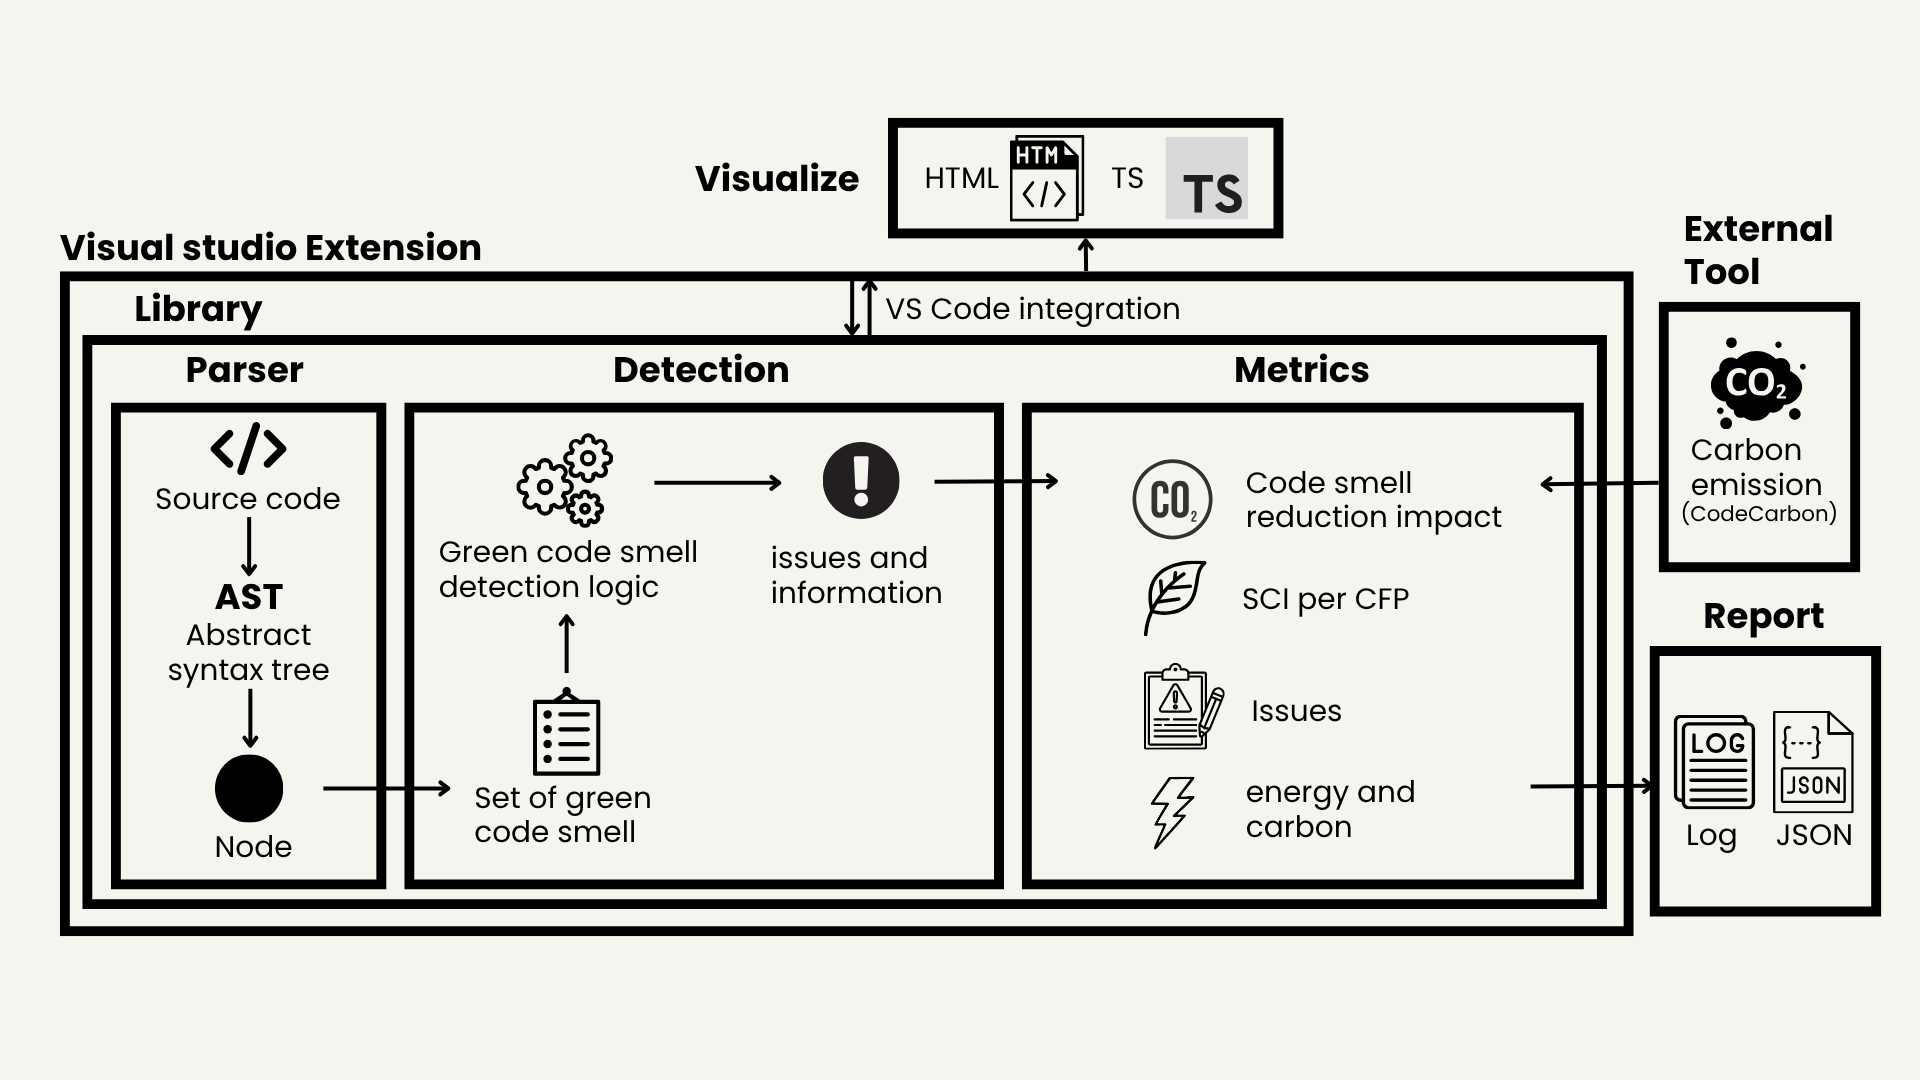
\includegraphics[width=\textwidth]{figures/chap4/Overall_SystemArchitecture.png}
\captionsetup{name=รูป}
\caption{สถาปัตยกรรมภาพรวมของระบบ PyGreenSense}
\label{fig:ch4_overall_architecture}
\end{figure}

รูป \ref{fig:ch4_overall_architecture} แสดงให้เห็นว่าตัวไลบรารีทำหน้าที่วิเคราะห์ซอร์สโค้ดและตรวจจับปัญหาเชิงโครงสร้าง ขณะที่ส่วนขยาย VS Code ทำหน้าที่เชื่อมการวิเคราะห์เข้าสู่ workflow ของผู้ใช้ และโมดูล Metrics ทำหน้าที่ประมวลผลข้อมูลด้านคาร์บอน พลังงาน CFP และผลกระทบจากการลด Code Smell เพื่อให้รายงานที่ได้มีทั้งมิติด้านคุณภาพโค้ดและความยั่งยืน

\subsection{AST Parser}
AST Parser ทำหน้าที่แปลงซอร์สโค้ดภาษา Python ให้อยู่ในรูปของโครงสร้าง {\italicfont Abstract Syntax Tree (AST)} โดยใช้โมดูล \texttt{ast} ของภาษา Python เพื่อให้สามารถวิเคราะห์องค์ประกอบของโปรแกรมในระดับโหนด เช่น ฟังก์ชัน คลาส ลูป การกำหนดค่า และการเรียกใช้ฟังก์ชันได้อย่างเป็นระบบ โครงสร้างดังกล่าวเป็นพื้นฐานสำคัญสำหรับการตรวจจับ Green Code Smell ในโครงงานนี้



\subsection{ชุดกฎ Green Code Smell}
ชุดกฎการตรวจจับถูกออกแบบขึ้นเพื่อระบุรูปแบบโค้ดที่อาจส่งผลต่อประสิทธิภาพด้านพลังงาน โดยอ้างอิงจากแนวคิดด้าน {\italicfont Green Software Engineering} งานวิจัยที่เกี่ยวข้อง และรายการ Green Code Smell ที่คัดเลือกมาใช้ในโครงงาน ได้แก่ {\italicfont Dead Code}, {\italicfont Long Method}, {\italicfont God Class}, {\italicfont Duplicated Code} และ {\italicfont Mutable Default Arguments}

\begin{table}[H]
\centering
\renewcommand{\arraystretch}{1.25}
\setlength{\tabcolsep}{6pt}
\begin{tabularx}{\textwidth}{|P{3.5cm}|X|}
\hline
{\boldfont Green Code Smell} & {\boldfont คำอธิบาย} \\
\hline
Dead Code & โค้ดที่ไม่ได้ถูกใช้งานจริง เช่น ตัวแปร ฟังก์ชัน คลาส หรือคำสั่งที่ไม่สามารถทำงานถึงได้ ({\italicfont unreachable code}) ซึ่งทำให้โค้ดมีส่วนเกินและเพิ่มภาระในการบำรุงรักษา รวมถึงอาจสะท้อนถึงการใช้ทรัพยากรที่ไม่จำเป็นในระบบ \cite{pylintUnreachable,pylintPossiblyUnusedVariable,vultureDeadCode,refactoringGuruDeadCode} \\
\hline
Long Method & ฟังก์ชันหรือเมธอดที่มีความยาวมากเกินไปและมีความซับซ้อนสูง โดยในโครงงานนี้พิจารณาจากจำนวนบรรทัดของโค้ดและค่า {\italicfont cyclomatic complexity} ซึ่งอาจทำให้โค้ดอ่านยาก ทดสอบยาก และเพิ่มภาระในการประมวลผล \cite{refactoringGuruLongMethod,guru99CyclomaticComplexity} \\
\hline
God Class & คลาสที่มีความรับผิดชอบมากเกินไป โดยในโครงงานนี้พิจารณาจากจำนวนบรรทัดของโค้ด ค่า {\italicfont cyclomatic complexity} และจำนวนเมธอดภายในคลาส ซึ่งมักสะท้อนถึงการรวมหลายหน้าที่ไว้ในคลาสเดียว \cite{refactoringGuruLargeClass,radonCyclomaticComplexity} \\
\hline
Duplicated Code & โค้ดที่มีความซ้ำคล้ายกันในหลายตำแหน่งของโปรแกรม โดยโครงงานนี้ใช้การเปรียบเทียบความคล้ายคลึงของโค้ดด้วย {\italicfont similarity threshold} เพื่อระบุกรณีที่มีการคัดลอกหรือเขียนซ้ำในลักษณะที่ใกล้เคียงกัน \cite{pythonDifflib,pylintDuplicateCode,refactoringGuruDuplicateCode} \\
\hline
Mutable Default Arguments & การกำหนดค่าเริ่มต้นของพารามิเตอร์ในฟังก์ชันเป็นชนิดข้อมูลที่เปลี่ยนแปลงได้ เช่น {\italicfont list}, {\italicfont dict} หรือ {\italicfont set} ซึ่งเป็น {\italicfont Python-specific code smell} ที่อาจทำให้เกิดพฤติกรรมไม่คาดคิดระหว่างการทำงาน \cite{pylintDangerousDefaultValue,sonarMutableDefaultArgument} \\
\hline
\end{tabularx}
\captionsetup{justification=centering, name=ตาราง}
\caption{Green Code Smell ที่สำคัญที่ใช้ในโครงการ}
\label{table:ch4_green_code_smells}
\end{table}

\subsubsection{ตรรกะการตรวจจับ Green Code Smell}
การตรวจจับ Green Code Smell ในโครงงานนี้ใช้การวิเคราะห์โครงสร้างซอร์สโค้ดภาษา Python ผ่าน Abstract Syntax Tree (AST) ร่วมกับพารามิเตอร์และเงื่อนไขที่กำหนดไว้ในแต่ละกฎ โดยแต่ละ Code Smell มีตรรกะการตรวจจับแตกต่างกันตามลักษณะของปัญหา ดังแสดงในตาราง \ref{table:ch4_detection_logic}

\begin{table}[H]
\centering
\scriptsize
\renewcommand{\arraystretch}{1.15}
\setlength{\tabcolsep}{4pt}
\begin{tabularx}{\textwidth}{|P{2.8cm}|P{3.6cm}|X|}
\hline
{\boldfont Code Smell} & {\boldfont Parameters} & {\boldfont Logic} \\
\hline

Long Method &
\texttt{max\_loc = 30}

\texttt{max\_cc = 10}
&
ตรวจสอบจำนวนบรรทัดโค้ด หรือ LOC และตรวจสอบค่าความซับซ้อนเชิงวัฏจักร หรือ Cyclomatic Complexity ของฟังก์ชัน หากจำนวนบรรทัดโค้ดหรือค่าความซับซ้อนเกินเกณฑ์ที่กำหนด ระบบจะนับเป็น Long Method \cite{refactoringGuruLongMethod,guru99CyclomaticComplexity}
\\
\hline

God Class &
\texttt{max\_cc = 35}

\texttt{max\_loc = 100}

\texttt{max\_methods = 10}
&
ตรวจสอบค่าความซับซ้อนเชิงวัฏจักร จำนวนบรรทัดโค้ด และจำนวนเมธอดภายในคลาส หากค่าใดค่าหนึ่งเกินเกณฑ์ที่กำหนด ระบบจะนับเป็น God Class \cite{refactoringGuruLargeClass,radonCyclomaticComplexity}
\\
\hline

Duplicated Code &
\texttt{similarity\_threshold = 0.85}
&
แปลงโค้ดให้อยู่ในรูปแบบมาตรฐาน เช่น แทนชื่อตัวแปรด้วย \texttt{VAR} และแทนค่าคงที่ด้วยประเภทของค่า จากนั้นเปรียบเทียบความคล้ายคลึงด้วย \texttt{difflib.SequenceMatcher} หากค่า Similarity Ratio สูงกว่า \texttt{0.85} จะนับเป็น Duplicated Code \cite{pythonDifflib,pylintDuplicateCode,refactoringGuruDuplicateCode}
\\
\hline

Dead Code &
ไม่มี parameter เฉพาะ
&
ตรวจสอบ 2 กรณีหลัก ได้แก่ Unused Variable และ Unreachable Code โดยใช้ AST เก็บข้อมูลส่วนที่ถูกประกาศและส่วนที่ถูกใช้งานจริง หากประกาศแต่ไม่ถูกใช้งานจะนับเป็น unused code และตรวจสอบคำสั่งที่ทำให้ flow สิ้นสุด เช่น \texttt{return}, \texttt{break}, \texttt{continue} และ \texttt{raise} เพื่อระบุ unreachable code \cite{pylintUnreachable,pylintPossiblyUnusedVariable,vultureDeadCode,refactoringGuruDeadCode}
\\
\hline

Mutable Default Arguments &
ไม่มี parameter เฉพาะ
&
ตรวจสอบ argument ของฟังก์ชันที่มีการกำหนดค่าเริ่มต้น และตรวจสอบว่าค่าเริ่มต้นนั้นเป็นชนิดข้อมูลที่เปลี่ยนแปลงได้หรือไม่ เช่น \texttt{list}, \texttt{dict} หรือ \texttt{set} หากพบ object ประเภทดังกล่าว ระบบจะนับเป็น Mutable Default Arguments \cite{pylintDangerousDefaultValue,sonarMutableDefaultArgument}
\\
\hline

\end{tabularx}
\captionsetup{justification=centering, name=ตาราง}
\caption{ตรรกะและพารามิเตอร์ที่ใช้ในการตรวจจับ Green Code Smell}
\label{table:ch4_detection_logic}
\end{table}

ความซับซ้อนเชิงวัฏจักร หรือ {\italicfont Cyclomatic Complexity} คือค่าที่ใช้ประเมินความซับซ้อนของเส้นทางการทำงานภายในโค้ด โดยพิจารณาจากโครงสร้างควบคุม เช่น loop, condition, \texttt{with}, list/dict/set comprehension และ operator ต่าง ๆ ยิ่งค่าดังกล่าวสูง โค้ดยิ่งมีเส้นทางการทำงานมากขึ้น และมักส่งผลให้การทดสอบ การบำรุงรักษา และการทำความเข้าใจโค้ดทำได้ยากขึ้น \cite{guru99CyclomaticComplexity,radonCyclomaticComplexity}

\subsection{VS Code Extension Module}
ส่วนขยาย VS Code ของโครงงานนี้ถูกพัฒนาขึ้นเพื่อทำหน้าที่เป็นส่วนติดต่อระหว่างผู้ใช้กับไลบรารีตรวจจับ Green Code Smell สำหรับภาษา Python โดยรองรับการเรียกใช้งานจากภายในสภาพแวดล้อมการพัฒนาโดยตรง ทำให้ผู้ใช้สามารถวิเคราะห์โค้ดและตรวจสอบผลลัพธ์ได้โดยไม่ต้องสลับไปใช้งานเครื่องมือภายนอก

ในเชิงโครงสร้าง ส่วนขยายถูกออกแบบให้มีคำสั่งหลักสำหรับการตรวจสอบสภาพแวดล้อมเสมือน การติดตั้ง dependency ที่จำเป็น การวิเคราะห์ไฟล์เดี่ยว และการวิเคราะห์ทั้งโปรเจกต์ โดยผู้ใช้สามารถเรียกใช้งานคำสั่งเหล่านี้ผ่าน Command Palette ของ VS Code ได้โดยตรง

ด้านการจัดการสภาพแวดล้อมการทำงาน ส่วนขยายใช้แนวทาง {\italicfont extension-managed virtual environment} โดยจัดเก็บ Python virtual environment ไว้ภายใต้พื้นที่จัดเก็บของส่วนขยายเอง ทำให้สามารถควบคุม dependency ที่เกี่ยวข้องกับระบบได้อย่างเป็นอิสระจากโปรเจกต์ของผู้ใช้ เมื่อระบบตรวจพบว่ายังไม่มี environment ที่พร้อมใช้งาน จะดำเนินการค้นหา system Python เพื่อใช้สร้าง virtual environment และติดตั้ง dependency ที่จำเป็นโดยอัตโนมัติ

ในการวิเคราะห์ ส่วนขยายจะตรวจสอบก่อนว่า CLI module ของ PyGreenSense สามารถเรียกใช้งานได้จริงใน environment ที่เตรียมไว้ หลังจากนั้นจึงเริ่มการวิเคราะห์ไฟล์หรือโปรเจกต์ตามขอบเขตที่ผู้ใช้เลือก โดยผลลัพธ์จากการวิเคราะห์จะถูกเก็บทั้งในรูปแบบข้อความจาก standard output และข้อมูลเชิงโครงสร้างที่บันทึกไว้ในไฟล์ \texttt{history.json} เพื่อรองรับการอ่านผลย้อนหลังและการเปรียบเทียบผลลัพธ์ระหว่างการรันแต่ละครั้ง

\subsection{Reporting Module}
โมดูลนี้ทำหน้าที่สรุปผลการตรวจสอบในรูปแบบรายงาน โดยแสดงประเภทของ Green Code Smell ตำแหน่งที่พบ ระดับความรุนแรง ค่าประมาณการใช้พลังงาน ปริมาณคาร์บอน และมาตรวัดเชิงฟังก์ชันที่เกี่ยวข้อง เช่น CFP และ SCI per CFP นอกจากนี้ยังรองรับการแสดงผลการเปรียบเทียบก่อนและหลังการปรับปรุง เพื่อช่วยให้ผู้ใช้เห็นผลของการแก้ไขโค้ดได้อย่างเป็นรูปธรรม

% -----------------------------------------------------

\section{การปฏิบัติ}

การพัฒนาโครงงานแบ่งออกเป็น 3 ระยะหลัก ได้แก่ การศึกษางานวิจัยพื้นฐาน การพัฒนาไลบรารีตรวจจับ Green Code Smell และการพัฒนาส่วนขยาย VS Code โดยมีรายละเอียดดังนี้

\subsection{ระยะการศึกษางานวิจัยและข้อมูลพื้นฐาน}
ในระยะนี้ ผู้พัฒนาได้ศึกษาทฤษฎีและงานวิจัยที่เกี่ยวข้องกับ Green Software Engineering, Code Smell, Software Carbon Intensity (SCI), CodeCarbon และ Cosmic Function Points (CFP) เพื่อใช้เป็นพื้นฐานในการออกแบบกฎตรวจจับ กลไกการวัดผล และรูปแบบการแสดงผลของระบบ

\subsection{ระยะการพัฒนาไลบรารีตรวจจับ Green Code Smell}
ในระยะนี้มีการปรับปรุงตรรกะการตรวจจับให้มีความยืดหยุ่นและแม่นยำมากขึ้น โดยประกอบด้วยการพัฒนาส่วนสำคัญดังนี้

\begin{itemize}
    \item {\boldfont Cross-file Dead Code Detection}: พัฒนาให้ระบบสามารถวิเคราะห์โหนด AST ข้ามหลายไฟล์ภายในโปรเจกต์ เพื่อประเมินสถานะการใช้งานของฟังก์ชัน ตัวแปร หรือองค์ประกอบอื่น ๆ ในระดับโปรเจกต์

    \item {\boldfont Enhanced Duplicated Code Logic}: ปรับปรุงอัลกอริทึมการเปรียบเทียบโครงสร้าง AST เพื่อให้สามารถตรวจจับโค้ดซ้ำได้แม่นยำขึ้น แม้จะมีการเปลี่ยนชื่อของตัวแปรหรือพารามิเตอร์

    \item {\boldfont Carbon-Smell Breakdown Engine}: พัฒนาระบบประมวลผลข้อมูลเพื่อคำนวณและเปรียบเทียบสัดส่วนผลกระทบของ Green Code Smell แต่ละประเภทตามสูตร Estimated Saving
\end{itemize}

ภาพรวมของ workflow ภายในไลบรารีแสดงในรูป \ref{fig:ch4_library_workflow} ซึ่งชี้ให้เห็นว่าขั้นตอนการทำงานเริ่มจากการรับซอร์สโค้ด การ parse และวิเคราะห์โครงสร้าง ก่อนวิ่งผ่านชุดกฎตรวจจับทีละประเภทและสรุปผลร่วมกับ metric ที่เกี่ยวข้อง

\begin{figure}[H]
\centering
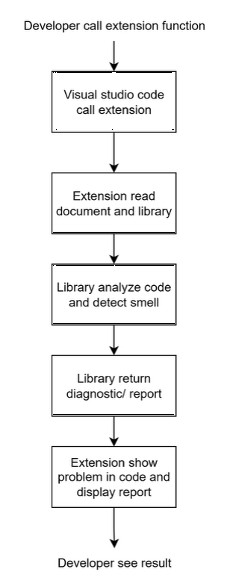
\includegraphics[width=0.45\textwidth]{figures/chap4/Process_Library.jpg}
\captionsetup{name=รูป}
\caption{Workflow การทำงานของไลบรารี PyGreenSense}
\label{fig:ch4_library_workflow}
\end{figure}

\subsection{ระยะการพัฒนาส่วนขยาย VS Code}
เมื่อไลบรารีตรวจจับพร้อมใช้งานแล้ว จึงพัฒนาส่วนขยาย VS Code เพื่อให้ผู้ใช้สามารถเข้าถึงผลการวิเคราะห์ได้สะดวกและตีความผลลัพธ์ได้ง่ายขึ้น โดยมีการพัฒนาสำคัญดังนี้

\begin{itemize}
    \item {\boldfont Library Deployment}
    
    เชื่อมต่อส่วนขยายกับไลบรารีที่ใช้งานจริงผ่านกลไก command bridge เพื่อให้ Extension สามารถสั่งรันโมดูลวิเคราะห์ รับค่าผลลัพธ์จากระบบตรวจจับ และดึงข้อมูลจากโมดูล Metric and Analysis ได้โดยตรง

    \item {\boldfont Advanced Visualization Dashboard}
    
    ออกแบบการแสดงผลข้อมูลจากไฟล์ JSON ให้อยู่ในรูปแบบ dashboard ที่เข้าใจง่าย เช่น กราฟเปรียบเทียบผลก่อนและหลังการปรับปรุง ({\italicfont Before vs After}) และแผนภูมิสัดส่วนผลกระทบรายประเภทของ Code Smell
\end{itemize}

ลำดับการทำงานของส่วนขยาย VS Code แสดงในรูป \ref{fig:ch4_extension_workflow} โดยผู้ใช้เริ่มต้นจากการเรียกคำสั่งของ Extension จากนั้นส่วนขยายจะอ่านเอกสารและเรียกใช้ไลบรารีเพื่อวิเคราะห์โค้ด ก่อนนำผลลัพธ์กลับมาแสดงทั้งในรูปแบบปัญหาบนโค้ดและรายงานสรุปภายใน VS Code

\begin{figure}[H]
\centering
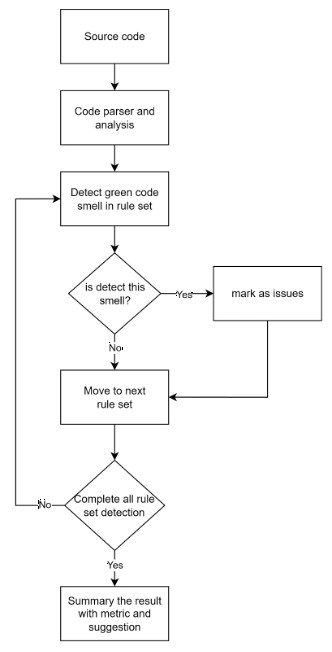
\includegraphics[width=0.32\textwidth]{figures/chap4/Process_VisualCodeExtension.jpg}
\captionsetup{name=รูป}
\caption{Workflow การทำงานของส่วนขยาย VS Code}
\label{fig:ch4_extension_workflow}
\end{figure}

% -----------------------------------------------------

\section{การทดสอบระบบ}

การทดสอบระบบมีวัตถุประสงค์เพื่อประเมินความถูกต้อง ความเสถียร และความเหมาะสมในการใช้งานจริงของทั้งไลบรารีและส่วนขยาย VS Code โดยแบ่งการทดสอบออกเป็นหลายด้านดังนี้

\subsection{การทดสอบไลบรารี}
มุ่งเน้นการทดสอบความถูกต้องของกฎตรวจจับ Green Code Smell แต่ละประเภท รวมถึงการทำงานร่วมกันของโมดูล AST Parser, Detection Rules และโมดูลคำนวณผลลัพธ์

\subsection{การทดสอบส่วนขยาย VS Code}
มุ่งเน้นการประเมินประสบการณ์ผู้ใช้ ความถูกต้องของข้อมูลที่แสดงผล และความสามารถในการเชื่อมต่อกับไลบรารีและระบบบันทึกผล

\subsection{การทดสอบด้านมาตรวัด}
ในส่วนนี้เน้นการตรวจสอบความถูกต้องของตรรกะการคำนวณมาตรวัดเชิงฟังก์ชัน มาตรวัดความเข้มข้นคาร์บอน และผลกระทบด้านการลดคาร์บอน โดยแยกการทดสอบออกเป็น 4 ส่วนสำคัญ เพื่อไม่ให้ตรรกะ CFP และ SCI ปะปนกับตรรกะการคำนวณสัดส่วน Carbon Saving ดังนี้

\begin{itemize}
    \item {\boldfont CFP Measurement Test}
    
    ทดสอบความถูกต้องของตรรกะการนับหน่วยฟังก์ชันของซอฟต์แวร์ หรือ Cosmic Function Points (CFP) โดยพิจารณาจากการระบุและนับจำนวนการเคลื่อนย้ายข้อมูล ({\italicfont Data Movements}) ได้แก่ Entry, Exit, Read และ Write เพื่อประเมินว่าระบบสามารถประมาณค่าขนาดเชิงฟังก์ชันของซอฟต์แวร์จากซอร์สโค้ดได้อย่างเหมาะสม

    \item {\boldfont SCI per CFP Measurement Test}
    
    ทดสอบตรรกะการคำนวณค่า Software Carbon Intensity ต่อหน่วย CFP หรือ {\italicfont SCI per CFP} โดยพิจารณาความสัมพันธ์ระหว่างปริมาณคาร์บอนที่ปล่อยออกมาและจำนวนหน่วยฟังก์ชันที่ระบบประมาณได้ เพื่อประเมินความเข้มข้นของคาร์บอนต่อหน่วยงานที่ซอฟต์แวร์ทำจริง

    \item {\boldfont Carbon Saving Impact Analysis Test}
    
    ทดสอบตรรกะการคำนวณสัดส่วนการประหยัดคาร์บอนจากข้อมูลที่จัดเก็บใน History Log โดยเปรียบเทียบข้อมูลก่อนและหลังการปรับปรุงโค้ด เช่น ปริมาณคาร์บอนรวม จำนวน Code Smell ที่ลดลง และจำนวนบรรทัดของโค้ดที่ถูกลบหรือปรับปรุงออกจากแต่ละกฎ เพื่อนำไปใช้ประเมินผลกระทบของการกำจัด Green Code Smell ต่อการลดปริมาณคาร์บอนในภาพรวม

    \item {\boldfont Inversion Case Handling}
    
    วิเคราะห์กรณีที่จำนวน CFP ลดลงในสัดส่วนที่มากกว่าปริมาณคาร์บอนที่ลดลง ซึ่งอาจทำให้ค่า SCI ต่อหน่วยสูงขึ้น แม้ว่าปริมาณคาร์บอนรวมจะลดลงก็ตาม กรณีนี้ใช้เพื่อตรวจสอบว่าระบบสามารถอธิบายผลลัพธ์ที่ดูขัดแย้งกันระหว่างคาร์บอนรวมและคาร์บอนต่อหน่วยฟังก์ชันได้อย่างถูกต้อง
\end{itemize}

ผลลัพธ์จากการทดสอบทั้ง 4 ส่วนถูกนำไปใช้กำหนดตรรกะการแสดงผลของระบบในบทประเมินผล โดยเฉพาะกรณี {\italicfont Inversion Case} ซึ่งช่วยให้ระบบอธิบายสถานการณ์ที่จำนวน Code Smell และ CFP ลดลง แต่ค่า SCI ต่อหน่วยกลับเพิ่มขึ้นได้อย่างเป็นระบบมากขึ้น ทั้งนี้ตัวอย่างผลการเปรียบเทียบจากการทดสอบจริงของไลบรารี ส่วนขยาย และข้อมูลจาก history log จะนำเสนอเพิ่มเติมในบทที่ \ref{Ch:Evaluation}
